\documentclass[a4paper]{book}
\usepackage{makeidx}
\usepackage{graphicx}
\usepackage{multicol}
\usepackage{float}
\usepackage{listings}
\usepackage{color}
\usepackage{ifthen}
\usepackage[table]{xcolor}
\usepackage{textcomp}
\usepackage{alltt}
\usepackage{ifpdf}
\ifpdf
\usepackage[pdftex,
            pagebackref=true,
            colorlinks=true,
            linkcolor=blue,
            unicode
           ]{hyperref}
\else
\usepackage[ps2pdf,
            pagebackref=true,
            colorlinks=true,
            linkcolor=blue,
            unicode
           ]{hyperref}
\usepackage{pspicture}
\fi
\usepackage[utf8]{inputenc}
\usepackage[french]{babel}

\usepackage{mathptmx}
\usepackage[scaled=.90]{helvet}
\usepackage{courier}
\usepackage{sectsty}
\usepackage[titles]{tocloft}
\usepackage{doxygen}
\lstset{language=C++,inputencoding=utf8,basicstyle=\footnotesize,breaklines=true,breakatwhitespace=true,tabsize=8,numbers=left }
\makeindex
\setcounter{tocdepth}{3}
\renewcommand{\footrulewidth}{0.4pt}
\renewcommand{\familydefault}{\sfdefault}
\begin{document}
\hypersetup{pageanchor=false}
\begin{titlepage}
\vspace*{7cm}
\begin{center}
{\Large Manuel de référence}\\
\vspace*{1cm}
{\large Généré par Doxygen 1.7.4}\\
\vspace*{0.5cm}
{\small Sun May 15 2011 16:14:39}\\
\end{center}
\end{titlepage}
\clearemptydoublepage
\pagenumbering{roman}
\tableofcontents
\clearemptydoublepage
\pagenumbering{arabic}
\hypersetup{pageanchor=true}
\chapter{Index des classes}
\section{Hiérarchie des classes}
Cette liste d'héritage est classée approximativement par ordre alphabétique :\begin{DoxyCompactList}
\item \contentsline{section}{FonctionTransfert}{\pageref{classFonctionTransfert}}{}
\begin{DoxyCompactList}
\item \contentsline{section}{Sigmoide}{\pageref{classSigmoide}}{}
\end{DoxyCompactList}
\item \contentsline{section}{IHM}{\pageref{classIHM}}{}
\item \contentsline{section}{Image}{\pageref{classImage}}{}
\item \contentsline{section}{Neurone}{\pageref{classNeurone}}{}
\begin{DoxyCompactList}
\item \contentsline{section}{NeuroneChainee}{\pageref{classNeuroneChainee}}{}
\end{DoxyCompactList}
\item \contentsline{section}{ReseauNeurone}{\pageref{classReseauNeurone}}{}
\begin{DoxyCompactList}
\item \contentsline{section}{ReseauNeuronesChainees}{\pageref{classReseauNeuronesChainees}}{}
\item \contentsline{section}{ReseauNeuronesCouches}{\pageref{classReseauNeuronesCouches}}{}
\end{DoxyCompactList}
\item \contentsline{section}{ReseauNeuroneChainees}{\pageref{classReseauNeuroneChainees}}{}
\end{DoxyCompactList}

\chapter{Index des classes}
\section{Liste des classes}
Liste des classes, structures, unions et interfaces avec une brève description :\begin{DoxyCompactList}
\item\contentsline{section}{\hyperlink{classFonctionTransfert}{FonctionTransfert} (Class \hyperlink{classFonctionTransfert}{FonctionTransfert} -\/ )}{\pageref{classFonctionTransfert}}{}
\item\contentsline{section}{\hyperlink{classIHM}{IHM} (Cette classe a pour but de charger l'interface en mode console )}{\pageref{classIHM}}{}
\item\contentsline{section}{\hyperlink{classImage}{Image} (Cette classe a pour but de charger facilement des images et de réaliser des traitements basiques dessus )}{\pageref{classImage}}{}
\item\contentsline{section}{\hyperlink{classNeurone}{Neurone} }{\pageref{classNeurone}}{}
\item\contentsline{section}{\hyperlink{classNeuroneChainee}{NeuroneChainee} }{\pageref{classNeuroneChainee}}{}
\item\contentsline{section}{\hyperlink{classReseauNeurone}{ReseauNeurone} }{\pageref{classReseauNeurone}}{}
\item\contentsline{section}{\hyperlink{classReseauNeuroneChainees}{ReseauNeuroneChainees} }{\pageref{classReseauNeuroneChainees}}{}
\item\contentsline{section}{\hyperlink{classReseauNeuronesChainees}{ReseauNeuronesChainees} }{\pageref{classReseauNeuronesChainees}}{}
\item\contentsline{section}{\hyperlink{classReseauNeuronesCouches}{ReseauNeuronesCouches} }{\pageref{classReseauNeuronesCouches}}{}
\item\contentsline{section}{\hyperlink{classSigmoide}{Sigmoide} (Class Sigmoïde -\/ )}{\pageref{classSigmoide}}{}
\end{DoxyCompactList}

\chapter{Documentation des classes}
\hypertarget{classFonctionTransfert}{
\section{Référence de la classe FonctionTransfert}
\label{classFonctionTransfert}\index{FonctionTransfert@{FonctionTransfert}}
}


class \hyperlink{classFonctionTransfert}{FonctionTransfert} -\/  




{\ttfamily \#include $<$FonctionTransfert.h$>$}

Graphe d'héritage de FonctionTransfert:\begin{figure}[H]
\begin{center}
\leavevmode
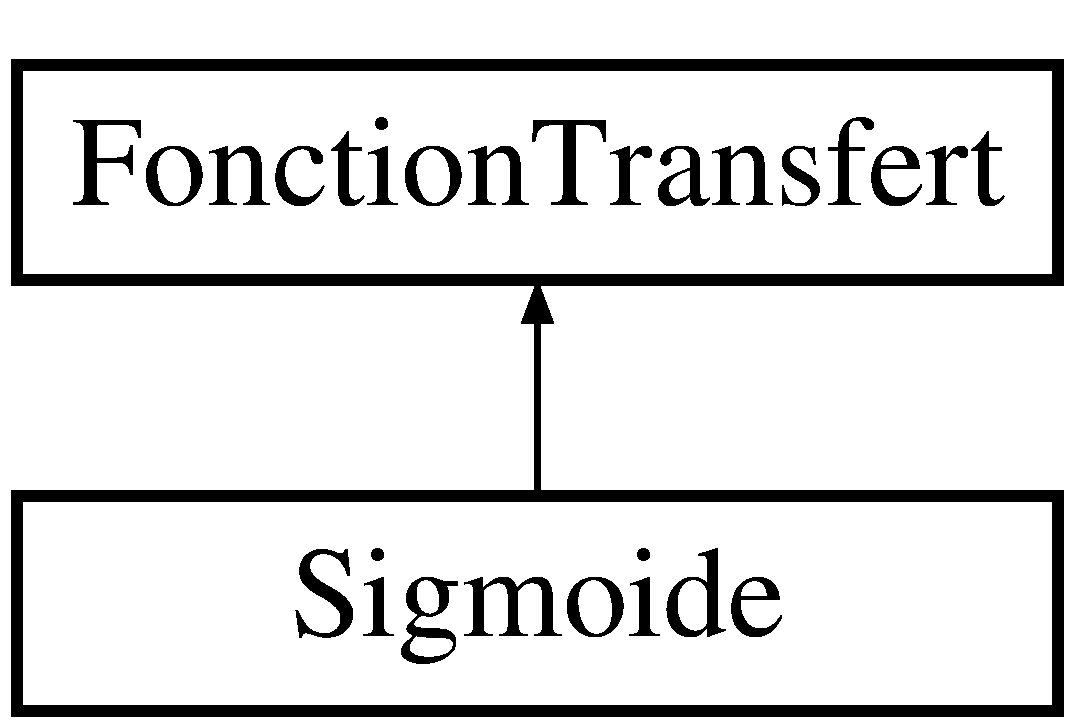
\includegraphics[height=2.000000cm]{classFonctionTransfert}
\end{center}
\end{figure}
\subsection*{Fonctions membres publiques}
\begin{DoxyCompactItemize}
\item 
\hypertarget{classFonctionTransfert_a6ddac1c50866b849bd7ae2f11caa2041}{
double {\bfseries f} (double x)}
\label{classFonctionTransfert_a6ddac1c50866b849bd7ae2f11caa2041}

\item 
\hypertarget{classFonctionTransfert_a095ee7763431d3253458d6b6f58582c5}{
double {\bfseries f\_\-inverse} (double x)}
\label{classFonctionTransfert_a095ee7763431d3253458d6b6f58582c5}

\end{DoxyCompactItemize}


\subsection{Description détaillée}
class \hyperlink{classFonctionTransfert}{FonctionTransfert} -\/ 

La documentation de cette classe a été générée à partir du fichier suivant :\begin{DoxyCompactItemize}
\item 
/home/cocouf/Documents/gm4/gm11-\/neurones/src/FonctionTransfert.h\end{DoxyCompactItemize}

\hypertarget{classIHM}{
\section{Référence de la classe IHM}
\label{classIHM}\index{IHM@{IHM}}
}


Cette classe a pour but de charger l'interface en mode console.  




{\ttfamily \#include $<$IHM.h$>$}

\subsection*{Fonctions membres publiques}
\begin{DoxyCompactItemize}
\item 
\hyperlink{classIHM_aade5baff871034cb667f43930620c121}{IHM} ()
\item 
\hyperlink{classIHM_af220622a4304f5a9ed1da28abb7da14d}{$\sim$IHM} ()
\item 
void \hyperlink{classIHM_acb3de40a81044c13b69dafac08465341}{menu} ()
\end{DoxyCompactItemize}


\subsection{Description détaillée}
Cette classe a pour but de charger l'interface en mode console. 

\subsection{Documentation des constructeurs et destructeur}
\hypertarget{classIHM_aade5baff871034cb667f43930620c121}{
\index{IHM@{IHM}!IHM@{IHM}}
\index{IHM@{IHM}!IHM@{IHM}}
\subsubsection[{IHM}]{\setlength{\rightskip}{0pt plus 5cm}IHM::IHM (
\begin{DoxyParamCaption}
{}
\end{DoxyParamCaption}
)}}
\label{classIHM_aade5baff871034cb667f43930620c121}
Ceci est le constructeur par defaut de la classe \hyperlink{classIHM}{IHM}. \hypertarget{classIHM_af220622a4304f5a9ed1da28abb7da14d}{
\index{IHM@{IHM}!$\sim$IHM@{$\sim$IHM}}
\index{$\sim$IHM@{$\sim$IHM}!IHM@{IHM}}
\subsubsection[{$\sim$IHM}]{\setlength{\rightskip}{0pt plus 5cm}IHM::$\sim$IHM (
\begin{DoxyParamCaption}
{}
\end{DoxyParamCaption}
)}}
\label{classIHM_af220622a4304f5a9ed1da28abb7da14d}
Ceci est le destructeur par defaut. 

\subsection{Documentation des fonctions membres}
\hypertarget{classIHM_acb3de40a81044c13b69dafac08465341}{
\index{IHM@{IHM}!menu@{menu}}
\index{menu@{menu}!IHM@{IHM}}
\subsubsection[{menu}]{\setlength{\rightskip}{0pt plus 5cm}void IHM::menu (
\begin{DoxyParamCaption}
{}
\end{DoxyParamCaption}
)}}
\label{classIHM_acb3de40a81044c13b69dafac08465341}
Lance le menu principal de l'interface. 

La documentation de cette classe a été générée à partir des fichiers suivants :\begin{DoxyCompactItemize}
\item 
/home/cocouf/Documents/gm4/gm11-\/neurones/src/IHM.h\item 
/home/cocouf/Documents/gm4/gm11-\/neurones/src/IHM.cpp\end{DoxyCompactItemize}

\hypertarget{classImage}{
\section{Référence de la classe Image}
\label{classImage}\index{Image@{Image}}
}


Cette classe a pour but de charger facilement des images et de réaliser des traitements basiques dessus.  




{\ttfamily \#include $<$Image.h$>$}

\subsection*{Fonctions membres publiques}
\begin{DoxyCompactItemize}
\item 
\hyperlink{classImage_ab5a8cd26aa2d32873ab871eef30bedf3}{Image} (string path)
\item 
\hyperlink{classImage_a0294f63700543e11c0f0da85601c7ae5}{$\sim$Image} ()
\item 
void \hyperlink{classImage_acf2a77d612bcbcfb91974dcfb484638c}{centerImage} ()
\item 
int \hyperlink{classImage_a2e162095e39208d81a694ec1db43de62}{obtenirPixel} (int x, int y)
\item 
vector$<$ double $>$ \hyperlink{classImage_a481a80ba76112618ef6a2320a40278af}{obtenirPixels} ()
\item 
vector$<$ int $>$ \hyperlink{classImage_ae07d3be7756c4bf735153a65b6281494}{LigneColonne} ()
\item 
\hypertarget{classImage_a4d957034ad17e3911a4d9f7decdda22c}{
void \hyperlink{classImage_a4d957034ad17e3911a4d9f7decdda22c}{afficher} ()}
\label{classImage_a4d957034ad17e3911a4d9f7decdda22c}

\begin{DoxyCompactList}\small\item\em Cette méthode permet d'afficher l'image jusqu'à ce que l'utilisateur ferme la fenêtre. \end{DoxyCompactList}\item 
\hypertarget{classImage_a490bfd3790cdd37f306e0e1751189e63}{
void \hyperlink{classImage_a490bfd3790cdd37f306e0e1751189e63}{afficher} (int n)}
\label{classImage_a490bfd3790cdd37f306e0e1751189e63}

\begin{DoxyCompactList}\small\item\em Cette méthode permet d'afficher l'image n millisecondes. \end{DoxyCompactList}\end{DoxyCompactItemize}
\subsection*{Amis}
\begin{DoxyCompactItemize}
\item 
\hypertarget{classImage_aba9b898604a39ecac2ab00c448e77a3a}{
class {\bfseries Image\_\-Test}}
\label{classImage_aba9b898604a39ecac2ab00c448e77a3a}

\end{DoxyCompactItemize}


\subsection{Description détaillée}
Cette classe a pour but de charger facilement des images et de réaliser des traitements basiques dessus. 

\subsection{Documentation des constructeurs et destructeur}
\hypertarget{classImage_ab5a8cd26aa2d32873ab871eef30bedf3}{
\index{Image@{Image}!Image@{Image}}
\index{Image@{Image}!Image@{Image}}
\subsubsection[{Image}]{\setlength{\rightskip}{0pt plus 5cm}Image::Image (
\begin{DoxyParamCaption}
\item[{string}]{path}
\end{DoxyParamCaption}
)}}
\label{classImage_ab5a8cd26aa2d32873ab871eef30bedf3}
Ceci est le constructeur de la classe \hyperlink{classImage}{Image} qui permet de charger une image. 
\begin{DoxyParams}{Paramètres}
{\em path} & le chemin (relatif) où se trouve l'image à charger \\
\hline
\end{DoxyParams}
\hypertarget{classImage_a0294f63700543e11c0f0da85601c7ae5}{
\index{Image@{Image}!$\sim$Image@{$\sim$Image}}
\index{$\sim$Image@{$\sim$Image}!Image@{Image}}
\subsubsection[{$\sim$Image}]{\setlength{\rightskip}{0pt plus 5cm}Image::$\sim$Image (
\begin{DoxyParamCaption}
{}
\end{DoxyParamCaption}
)}}
\label{classImage_a0294f63700543e11c0f0da85601c7ae5}
Ceci est le destructeur de la classe \hyperlink{classImage}{Image} qui permet de charger une image. 

\subsection{Documentation des fonctions membres}
\hypertarget{classImage_acf2a77d612bcbcfb91974dcfb484638c}{
\index{Image@{Image}!centerImage@{centerImage}}
\index{centerImage@{centerImage}!Image@{Image}}
\subsubsection[{centerImage}]{\setlength{\rightskip}{0pt plus 5cm}void Image::centerImage (
\begin{DoxyParamCaption}
{}
\end{DoxyParamCaption}
)}}
\label{classImage_acf2a77d612bcbcfb91974dcfb484638c}
Cette méthode a pour but de recentrer l'image dans l'optique d'un prétraitement. \hypertarget{classImage_ae07d3be7756c4bf735153a65b6281494}{
\index{Image@{Image}!LigneColonne@{LigneColonne}}
\index{LigneColonne@{LigneColonne}!Image@{Image}}
\subsubsection[{LigneColonne}]{\setlength{\rightskip}{0pt plus 5cm}std::vector$<$ int $>$ Image::LigneColonne (
\begin{DoxyParamCaption}
{}
\end{DoxyParamCaption}
)}}
\label{classImage_ae07d3be7756c4bf735153a65b6281494}
Cette méthode retourne la somme des pixels sur chaque ligne et colonne. \begin{DoxyReturn}{Renvoie}
renvois un tableau de données. 
\end{DoxyReturn}
\hypertarget{classImage_a2e162095e39208d81a694ec1db43de62}{
\index{Image@{Image}!obtenirPixel@{obtenirPixel}}
\index{obtenirPixel@{obtenirPixel}!Image@{Image}}
\subsubsection[{obtenirPixel}]{\setlength{\rightskip}{0pt plus 5cm}int Image::obtenirPixel (
\begin{DoxyParamCaption}
\item[{int}]{x, }
\item[{int}]{y}
\end{DoxyParamCaption}
)}}
\label{classImage_a2e162095e39208d81a694ec1db43de62}
Retourne la valeur du pixel souhaité 
\begin{DoxyParams}{Paramètres}
{\em x} & ordonnée du pixel \\
\hline
{\em y} & abscisse du pixel \\
\hline
\end{DoxyParams}
\hypertarget{classImage_a481a80ba76112618ef6a2320a40278af}{
\index{Image@{Image}!obtenirPixels@{obtenirPixels}}
\index{obtenirPixels@{obtenirPixels}!Image@{Image}}
\subsubsection[{obtenirPixels}]{\setlength{\rightskip}{0pt plus 5cm}vector$<$ double $>$ Image::obtenirPixels (
\begin{DoxyParamCaption}
{}
\end{DoxyParamCaption}
)}}
\label{classImage_a481a80ba76112618ef6a2320a40278af}
Retourne le tableau de pixels de l'image \begin{DoxyReturn}{Renvoie}
tableau avec tous les pixels. 
\end{DoxyReturn}


La documentation de cette classe a été générée à partir des fichiers suivants :\begin{DoxyCompactItemize}
\item 
/home/cocouf/Documents/gm4/gm11-\/neurones/src/Image.h\item 
/home/cocouf/Documents/gm4/gm11-\/neurones/src/Image.cpp\end{DoxyCompactItemize}

\hypertarget{classNeurone}{
\section{Référence de la classe Neurone}
\label{classNeurone}\index{Neurone@{Neurone}}
}
Graphe d'héritage de Neurone:\begin{figure}[H]
\begin{center}
\leavevmode
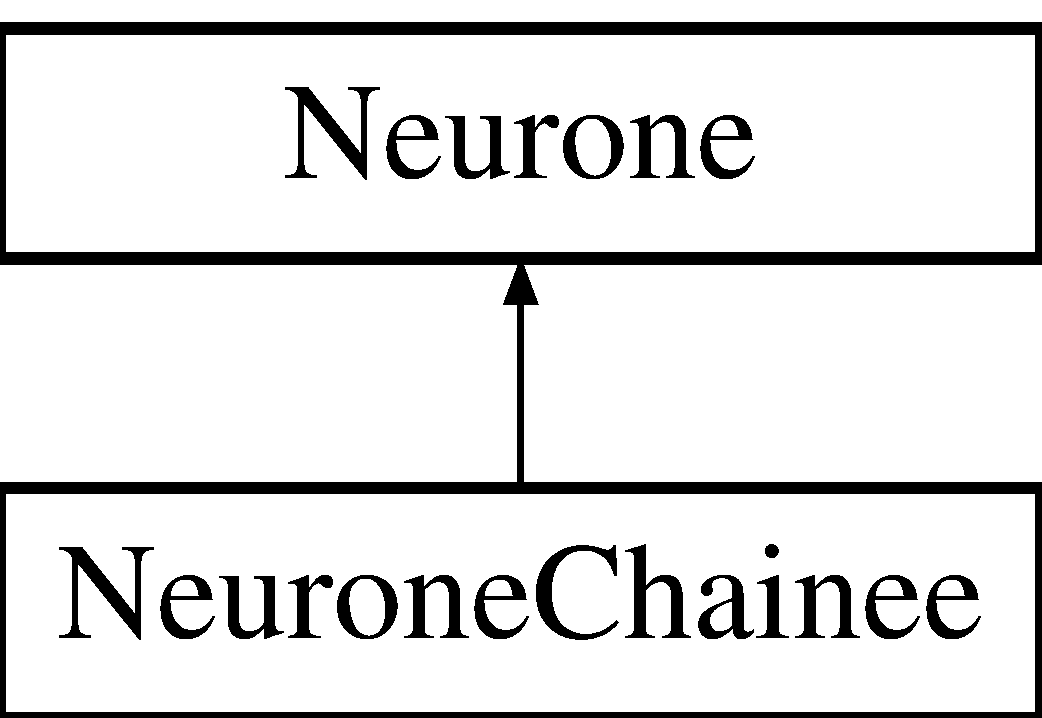
\includegraphics[height=2.000000cm]{classNeurone}
\end{center}
\end{figure}
\subsection*{Fonctions membres publiques}
\begin{DoxyCompactItemize}
\item 
\hyperlink{classNeurone_a8584aa9020d36c16e695b623daaf1776}{Neurone} (int identifiant, int nbAntecedents)
\begin{DoxyCompactList}\small\item\em Ceci est le créateur d'un neurone. \end{DoxyCompactList}\item 
\hypertarget{classNeurone_a82d4936ed8ac6c87cb07c117eca23953}{
{\bfseries Neurone} (const \hyperlink{classNeurone}{Neurone} \&n)}
\label{classNeurone_a82d4936ed8ac6c87cb07c117eca23953}

\item 
virtual void \hyperlink{classNeurone_aba7e64f609a6bf0d154ef1a6f6230be6}{chargerNeurone} (ifstream $\ast$sauvegarde)
\begin{DoxyCompactList}\small\item\em Cette méthode permet de lire un neurone dans un fichier. \end{DoxyCompactList}\item 
virtual void \hyperlink{classNeurone_a4e0c2a9243285ff1b5842792c95200d7}{sauvegarderNeurone} (ofstream $\ast$sauvegarde)
\begin{DoxyCompactList}\small\item\em Cette méthode permet de sauvegarder un neurone dans un fichier. \end{DoxyCompactList}\item 
virtual void \hyperlink{classNeurone_ae645e1d7f44e896df23103555a4bc660}{calculeValeurTransfert} (vector$<$ double $>$ entreeSynaptique)
\begin{DoxyCompactList}\small\item\em Calcule la valeur de transfert à partir des entrée synaptiques qui lui sont données. \end{DoxyCompactList}\item 
virtual double \hyperlink{classNeurone_a5bc0eb4b565fde75df3333ded397a4b1}{getValeurSortie} ()
\begin{DoxyCompactList}\small\item\em Cette méthode retourne la valeur de sortie du neurone après passage dans la fonction de transfert. \end{DoxyCompactList}\item 
virtual int \hyperlink{classNeurone_afca63a97bda3af1aa66e355af268d709}{getIdentifiant} ()
\begin{DoxyCompactList}\small\item\em Cette méthode retourne la valeur de l'identifiant du neurone. \end{DoxyCompactList}\item 
virtual void \hyperlink{classNeurone_a69db84522682c056696f55c772c85adb}{setValeurEntree} (double v)
\begin{DoxyCompactList}\small\item\em Permet d'assigner la valeur d'entrée du neurone (utile quand le neurone est de la première couche). \end{DoxyCompactList}\item 
virtual void \hyperlink{classNeurone_ac21b2c8c216ae35780120037fa49d428}{setPoidsSynaptic} (vector$<$ double $>$ poids)
\begin{DoxyCompactList}\small\item\em Permet d'assigner la valeur des poids synaptiques du neurone (pour la phase d'apprentissage). \end{DoxyCompactList}\item 
virtual vector$<$ double $>$ \hyperlink{classNeurone_ac360dcc14d2c4a3e4fd91d305c23ce7f}{getPoidsSynaptic} ()
\begin{DoxyCompactList}\small\item\em Permet de récupérer la valeur des poids synaptiques du neurone (pour la phase d'apprentissage). \end{DoxyCompactList}\item 
\hypertarget{classNeurone_a76611fb63e5deb9193020c141d1b3908}{
virtual double {\bfseries getValeurAvantTrasphert} ()}
\label{classNeurone_a76611fb63e5deb9193020c141d1b3908}

\end{DoxyCompactItemize}
\subsection*{Attributs protégés}
\begin{DoxyCompactItemize}
\item 
\hypertarget{classNeurone_a063243e7659e0536178213f0db85ed9f}{
int {\bfseries identifiant}}
\label{classNeurone_a063243e7659e0536178213f0db85ed9f}

\item 
\hypertarget{classNeurone_aba2837a2cfe54ad9ae6afa8f706212bb}{
double {\bfseries valeurTransfert}}
\label{classNeurone_aba2837a2cfe54ad9ae6afa8f706212bb}

\item 
\hypertarget{classNeurone_a27ba6b3bcda980aa40e154047905c6f7}{
double {\bfseries valeurErreur}}
\label{classNeurone_a27ba6b3bcda980aa40e154047905c6f7}

\item 
\hypertarget{classNeurone_a98851f89e12cbbec4983dc2b44156e4a}{
vector$<$ double $>$ {\bfseries poidsSynaptiques}}
\label{classNeurone_a98851f89e12cbbec4983dc2b44156e4a}

\item 
\hypertarget{classNeurone_a7dc2d1919d027b4d030f957262405d9f}{
\hyperlink{classFonctionTransfert}{FonctionTransfert} {\bfseries fonctionTransfert}}
\label{classNeurone_a7dc2d1919d027b4d030f957262405d9f}

\end{DoxyCompactItemize}
\subsection*{Amis}
\begin{DoxyCompactItemize}
\item 
\hypertarget{classNeurone_ad337320a77a70676ada0b514870dd529}{
class {\bfseries Test\_\-Neurone}}
\label{classNeurone_ad337320a77a70676ada0b514870dd529}

\item 
\hypertarget{classNeurone_a755d7d72d9539f75e09ce6a61ce5e702}{
class {\bfseries Test\_\-ReseauNeuronesCouche}}
\label{classNeurone_a755d7d72d9539f75e09ce6a61ce5e702}

\end{DoxyCompactItemize}


\subsection{Description détaillée}
représente un neurone. 

\subsection{Documentation des constructeurs et destructeur}
\hypertarget{classNeurone_a8584aa9020d36c16e695b623daaf1776}{
\index{Neurone@{Neurone}!Neurone@{Neurone}}
\index{Neurone@{Neurone}!Neurone@{Neurone}}
\subsubsection[{Neurone}]{\setlength{\rightskip}{0pt plus 5cm}Neurone::Neurone (
\begin{DoxyParamCaption}
\item[{int}]{identifiant, }
\item[{int}]{nbAntecedents}
\end{DoxyParamCaption}
)}}
\label{classNeurone_a8584aa9020d36c16e695b623daaf1776}


Ceci est le créateur d'un neurone. 


\begin{DoxyParams}{Paramètres}
{\em identifiant} & le numéro d'identification du neurone. \\
\hline
{\em nbAntecedents} & le nombre d'antecedents qu'aura le neurone (c'est à dire le nombre de coefficient synaptic qu'il aura) \\
\hline
\end{DoxyParams}


\subsection{Documentation des fonctions membres}
\hypertarget{classNeurone_ae645e1d7f44e896df23103555a4bc660}{
\index{Neurone@{Neurone}!calculeValeurTransfert@{calculeValeurTransfert}}
\index{calculeValeurTransfert@{calculeValeurTransfert}!Neurone@{Neurone}}
\subsubsection[{calculeValeurTransfert}]{\setlength{\rightskip}{0pt plus 5cm}void Neurone::calculeValeurTransfert (
\begin{DoxyParamCaption}
\item[{vector$<$ double $>$}]{entreeSynaptique}
\end{DoxyParamCaption}
)\hspace{0.3cm}{\ttfamily  \mbox{[}virtual\mbox{]}}}}
\label{classNeurone_ae645e1d7f44e896df23103555a4bc660}


Calcule la valeur de transfert à partir des entrée synaptiques qui lui sont données. 


\begin{DoxyParams}{Paramètres}
{\em entreeSynaptique} & donne les valeurs aux entrées du neurones. \\
\hline
\end{DoxyParams}
\hypertarget{classNeurone_aba7e64f609a6bf0d154ef1a6f6230be6}{
\index{Neurone@{Neurone}!chargerNeurone@{chargerNeurone}}
\index{chargerNeurone@{chargerNeurone}!Neurone@{Neurone}}
\subsubsection[{chargerNeurone}]{\setlength{\rightskip}{0pt plus 5cm}void Neurone::chargerNeurone (
\begin{DoxyParamCaption}
\item[{ifstream $\ast$}]{sauvegarde}
\end{DoxyParamCaption}
)\hspace{0.3cm}{\ttfamily  \mbox{[}virtual\mbox{]}}}}
\label{classNeurone_aba7e64f609a6bf0d154ef1a6f6230be6}


Cette méthode permet de lire un neurone dans un fichier. 


\begin{DoxyParams}{Paramètres}
{\em sauvegarde} & le fichier dans lequel il faut lire le neurone. \\
\hline
\end{DoxyParams}
\hypertarget{classNeurone_afca63a97bda3af1aa66e355af268d709}{
\index{Neurone@{Neurone}!getIdentifiant@{getIdentifiant}}
\index{getIdentifiant@{getIdentifiant}!Neurone@{Neurone}}
\subsubsection[{getIdentifiant}]{\setlength{\rightskip}{0pt plus 5cm}int Neurone::getIdentifiant (
\begin{DoxyParamCaption}
{}
\end{DoxyParamCaption}
)\hspace{0.3cm}{\ttfamily  \mbox{[}virtual\mbox{]}}}}
\label{classNeurone_afca63a97bda3af1aa66e355af268d709}


Cette méthode retourne la valeur de l'identifiant du neurone. 

\begin{DoxyReturn}{Renvoie}
l'identifiant du neurone. 
\end{DoxyReturn}
\hypertarget{classNeurone_ac360dcc14d2c4a3e4fd91d305c23ce7f}{
\index{Neurone@{Neurone}!getPoidsSynaptic@{getPoidsSynaptic}}
\index{getPoidsSynaptic@{getPoidsSynaptic}!Neurone@{Neurone}}
\subsubsection[{getPoidsSynaptic}]{\setlength{\rightskip}{0pt plus 5cm}std::vector$<$ double, std::allocator$<$ double $>$ $>$ Neurone::getPoidsSynaptic (
\begin{DoxyParamCaption}
{}
\end{DoxyParamCaption}
)\hspace{0.3cm}{\ttfamily  \mbox{[}virtual\mbox{]}}}}
\label{classNeurone_ac360dcc14d2c4a3e4fd91d305c23ce7f}


Permet de récupérer la valeur des poids synaptiques du neurone (pour la phase d'apprentissage). 

\begin{DoxyReturn}{Renvoie}
la valeur des poids. 
\end{DoxyReturn}
\hypertarget{classNeurone_a5bc0eb4b565fde75df3333ded397a4b1}{
\index{Neurone@{Neurone}!getValeurSortie@{getValeurSortie}}
\index{getValeurSortie@{getValeurSortie}!Neurone@{Neurone}}
\subsubsection[{getValeurSortie}]{\setlength{\rightskip}{0pt plus 5cm}double Neurone::getValeurSortie (
\begin{DoxyParamCaption}
{}
\end{DoxyParamCaption}
)\hspace{0.3cm}{\ttfamily  \mbox{[}virtual\mbox{]}}}}
\label{classNeurone_a5bc0eb4b565fde75df3333ded397a4b1}


Cette méthode retourne la valeur de sortie du neurone après passage dans la fonction de transfert. 

\begin{DoxyReturn}{Renvoie}
la valeur de sortie. 
\end{DoxyReturn}
\hypertarget{classNeurone_a4e0c2a9243285ff1b5842792c95200d7}{
\index{Neurone@{Neurone}!sauvegarderNeurone@{sauvegarderNeurone}}
\index{sauvegarderNeurone@{sauvegarderNeurone}!Neurone@{Neurone}}
\subsubsection[{sauvegarderNeurone}]{\setlength{\rightskip}{0pt plus 5cm}void Neurone::sauvegarderNeurone (
\begin{DoxyParamCaption}
\item[{ofstream $\ast$}]{sauvegarde}
\end{DoxyParamCaption}
)\hspace{0.3cm}{\ttfamily  \mbox{[}virtual\mbox{]}}}}
\label{classNeurone_a4e0c2a9243285ff1b5842792c95200d7}


Cette méthode permet de sauvegarder un neurone dans un fichier. 


\begin{DoxyParams}{Paramètres}
{\em sauvegarde} & le fichier dans lequel il faut écrire le neurone. \\
\hline
\end{DoxyParams}
\hypertarget{classNeurone_ac21b2c8c216ae35780120037fa49d428}{
\index{Neurone@{Neurone}!setPoidsSynaptic@{setPoidsSynaptic}}
\index{setPoidsSynaptic@{setPoidsSynaptic}!Neurone@{Neurone}}
\subsubsection[{setPoidsSynaptic}]{\setlength{\rightskip}{0pt plus 5cm}void Neurone::setPoidsSynaptic (
\begin{DoxyParamCaption}
\item[{vector$<$ double $>$}]{poids}
\end{DoxyParamCaption}
)\hspace{0.3cm}{\ttfamily  \mbox{[}virtual\mbox{]}}}}
\label{classNeurone_ac21b2c8c216ae35780120037fa49d428}


Permet d'assigner la valeur des poids synaptiques du neurone (pour la phase d'apprentissage). 


\begin{DoxyParams}{Paramètres}
{\em poids} & les valeurs souhaitées. \\
\hline
\end{DoxyParams}
\hypertarget{classNeurone_a69db84522682c056696f55c772c85adb}{
\index{Neurone@{Neurone}!setValeurEntree@{setValeurEntree}}
\index{setValeurEntree@{setValeurEntree}!Neurone@{Neurone}}
\subsubsection[{setValeurEntree}]{\setlength{\rightskip}{0pt plus 5cm}void Neurone::setValeurEntree (
\begin{DoxyParamCaption}
\item[{double}]{v}
\end{DoxyParamCaption}
)\hspace{0.3cm}{\ttfamily  \mbox{[}virtual\mbox{]}}}}
\label{classNeurone_a69db84522682c056696f55c772c85adb}


Permet d'assigner la valeur d'entrée du neurone (utile quand le neurone est de la première couche). 


\begin{DoxyParams}{Paramètres}
{\em v} & la valeur souhaitée. \\
\hline
\end{DoxyParams}


La documentation de cette classe a été générée à partir des fichiers suivants :\begin{DoxyCompactItemize}
\item 
/home/cocouf/Documents/gm4/gm11-\/neurones/src/Neurone.h\item 
/home/cocouf/Documents/gm4/gm11-\/neurones/src/Neurone.cpp\end{DoxyCompactItemize}

\hypertarget{classNeuroneChainee}{
\section{Référence de la classe NeuroneChainee}
\label{classNeuroneChainee}\index{NeuroneChainee@{NeuroneChainee}}
}
Graphe d'héritage de NeuroneChainee:\begin{figure}[H]
\begin{center}
\leavevmode
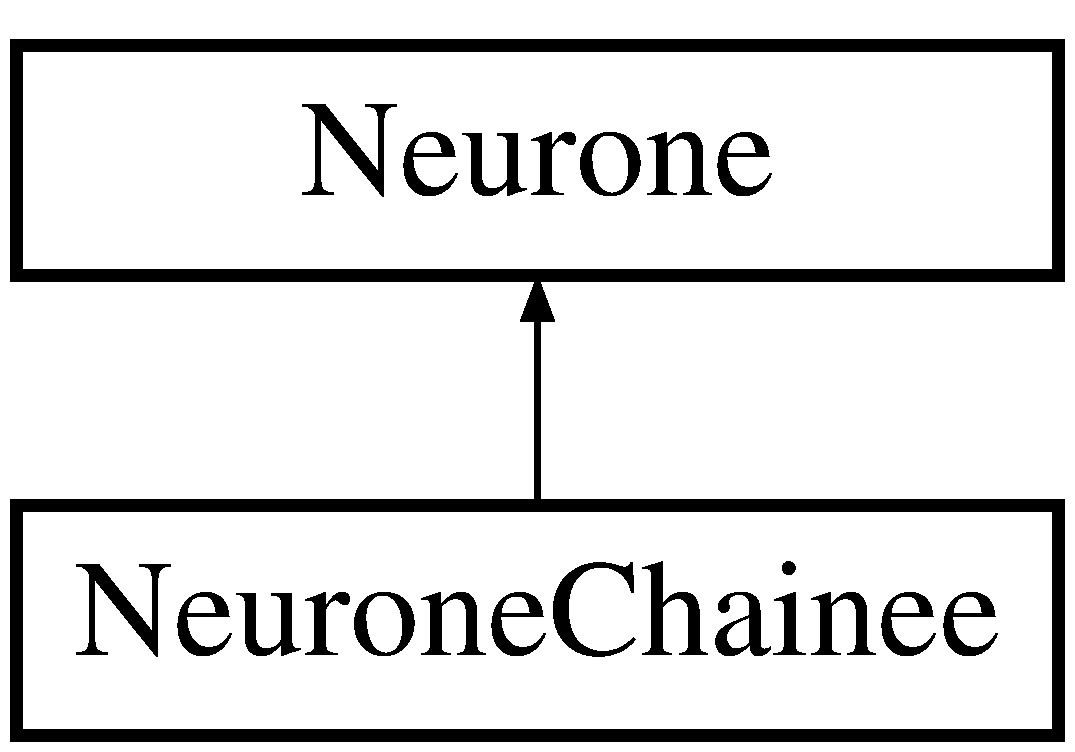
\includegraphics[height=2.000000cm]{classNeuroneChainee}
\end{center}
\end{figure}
\subsection*{Fonctions membres publiques}
\begin{DoxyCompactItemize}
\item 
double \hyperlink{classNeuroneChainee_a37157dd7511e23dfb2552e423cde0513}{calculerValeur} ()
\begin{DoxyCompactList}\small\item\em Cette méthode permet de calculer la valeur du neurone en faisant des appels récurcifs. La méthode calcule le resultat et la met dans la variable. \end{DoxyCompactList}\item 
double \hyperlink{classNeuroneChainee_a14ed4fce5282c1515d56edcfa6d89344}{calculerErreur} ()
\begin{DoxyCompactList}\small\item\em Cette méthode permet de calculer l'erreur du neurone en faisant des appels récurcifs. La méthode calcule le resultat et la met dans la variable. \end{DoxyCompactList}\end{DoxyCompactItemize}


\subsection{Description détaillée}
hérite de la classe neurone et permet de de réaliser des réseaux de neurones en graphe 

\subsection{Documentation des fonctions membres}
\hypertarget{classNeuroneChainee_a14ed4fce5282c1515d56edcfa6d89344}{
\index{NeuroneChainee@{NeuroneChainee}!calculerErreur@{calculerErreur}}
\index{calculerErreur@{calculerErreur}!NeuroneChainee@{NeuroneChainee}}
\subsubsection[{calculerErreur}]{\setlength{\rightskip}{0pt plus 5cm}double NeuroneChainee::calculerErreur (
\begin{DoxyParamCaption}
{}
\end{DoxyParamCaption}
)}}
\label{classNeuroneChainee_a14ed4fce5282c1515d56edcfa6d89344}


Cette méthode permet de calculer l'erreur du neurone en faisant des appels récurcifs. La méthode calcule le resultat et la met dans la variable. 

\begin{DoxyReturn}{Renvoie}
donne l'erreur. 
\end{DoxyReturn}
\hypertarget{classNeuroneChainee_a37157dd7511e23dfb2552e423cde0513}{
\index{NeuroneChainee@{NeuroneChainee}!calculerValeur@{calculerValeur}}
\index{calculerValeur@{calculerValeur}!NeuroneChainee@{NeuroneChainee}}
\subsubsection[{calculerValeur}]{\setlength{\rightskip}{0pt plus 5cm}double NeuroneChainee::calculerValeur (
\begin{DoxyParamCaption}
{}
\end{DoxyParamCaption}
)}}
\label{classNeuroneChainee_a37157dd7511e23dfb2552e423cde0513}


Cette méthode permet de calculer la valeur du neurone en faisant des appels récurcifs. La méthode calcule le resultat et la met dans la variable. 

\begin{DoxyReturn}{Renvoie}
donne la valeur. 
\end{DoxyReturn}


La documentation de cette classe a été générée à partir du fichier suivant :\begin{DoxyCompactItemize}
\item 
/home/cocouf/Documents/gm4/gm11-\/neurones/src/NeuroneChainee.h\end{DoxyCompactItemize}

\hypertarget{classReseauNeurone}{
\section{Référence de la classe ReseauNeurone}
\label{classReseauNeurone}\index{ReseauNeurone@{ReseauNeurone}}
}
Graphe d'héritage de ReseauNeurone:\begin{figure}[H]
\begin{center}
\leavevmode
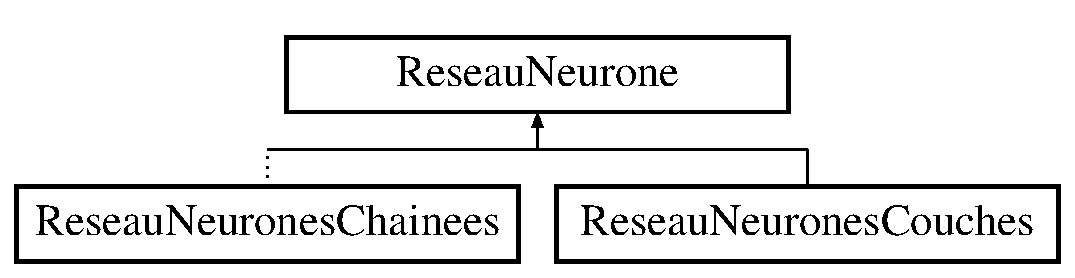
\includegraphics[height=2.000000cm]{classReseauNeurone}
\end{center}
\end{figure}
\subsection*{Fonctions membres publiques}
\begin{DoxyCompactItemize}
\item 
virtual bool \hyperlink{classReseauNeurone_ac2bccb9c9106a989960246e8f173d93a}{chargerReseau} (string path)=0
\begin{DoxyCompactList}\small\item\em Cette méthode permet de charger un réseau lu dans un fichier. \end{DoxyCompactList}\item 
virtual bool \hyperlink{classReseauNeurone_a33c828f2e2b7a190eff04c613707a9d4}{sauvegarderReseau} (string path)=0
\begin{DoxyCompactList}\small\item\em Cette méthode permet de sauvegarder un réseau dans un fichier. \end{DoxyCompactList}\item 
void \hyperlink{classReseauNeurone_ad29ad61f93877aaf2ee930106d46e48b}{apprendre} (vector$<$ double $>$ $\ast$entrees, vector$<$ double $>$ $\ast$valeursAttendues, int n)
\begin{DoxyCompactList}\small\item\em Cette méthode permet de réaliser une étape d'apprentissage. \end{DoxyCompactList}\item 
vector$<$ double $>$ \hyperlink{classReseauNeurone_add3e1d607bc614ca36b0375daf546106}{calculerResultat} (vector$<$ double $>$ valeurEntree)
\begin{DoxyCompactList}\small\item\em Cette méthode permet de calculer le résultat sur la couche de sortie. \end{DoxyCompactList}\end{DoxyCompactItemize}
\subsection*{Attributs protégés}
\begin{DoxyCompactItemize}
\item 
\hypertarget{classReseauNeurone_a330aab82b9bdef4e03f88522330eb10f}{
vector$<$ \hyperlink{classNeurone}{Neurone} $>$ {\bfseries Neurones}}
\label{classReseauNeurone_a330aab82b9bdef4e03f88522330eb10f}

\end{DoxyCompactItemize}


\subsection{Description détaillée}
représentant un réseau de neurones. 

\subsection{Documentation des fonctions membres}
\hypertarget{classReseauNeurone_ad29ad61f93877aaf2ee930106d46e48b}{
\index{ReseauNeurone@{ReseauNeurone}!apprendre@{apprendre}}
\index{apprendre@{apprendre}!ReseauNeurone@{ReseauNeurone}}
\subsubsection[{apprendre}]{\setlength{\rightskip}{0pt plus 5cm}void ReseauNeurone::apprendre (
\begin{DoxyParamCaption}
\item[{vector$<$ double $>$ $\ast$}]{entrees, }
\item[{vector$<$ double $>$ $\ast$}]{valeursAttendues, }
\item[{int}]{n}
\end{DoxyParamCaption}
)}}
\label{classReseauNeurone_ad29ad61f93877aaf2ee930106d46e48b}


Cette méthode permet de réaliser une étape d'apprentissage. 


\begin{DoxyParams}{Paramètres}
{\em entrees} & liste des entrées pour le jeu d'apprentiassage. \\
\hline
{\em valeursAttendues} & les valeurs attendues en sortie pour chacune de ses entrées. \\
\hline
{\em n} & la taille de l'échantillon d'apprentissage. \\
\hline
\end{DoxyParams}


Réimplémentée dans \hyperlink{classReseauNeuronesCouches_ad368a99d25583fd49d384516dacb3062}{ReseauNeuronesCouches}.

\hypertarget{classReseauNeurone_add3e1d607bc614ca36b0375daf546106}{
\index{ReseauNeurone@{ReseauNeurone}!calculerResultat@{calculerResultat}}
\index{calculerResultat@{calculerResultat}!ReseauNeurone@{ReseauNeurone}}
\subsubsection[{calculerResultat}]{\setlength{\rightskip}{0pt plus 5cm}vector$<$double$>$ ReseauNeurone::calculerResultat (
\begin{DoxyParamCaption}
\item[{vector$<$ double $>$}]{valeurEntree}
\end{DoxyParamCaption}
)}}
\label{classReseauNeurone_add3e1d607bc614ca36b0375daf546106}


Cette méthode permet de calculer le résultat sur la couche de sortie. 

\begin{DoxyReturn}{Renvoie}
la valeur des résultats. 
\end{DoxyReturn}


Réimplémentée dans \hyperlink{classReseauNeuronesCouches_ad2cb2070ae32e8772bf82e6d06221bdd}{ReseauNeuronesCouches}.

\hypertarget{classReseauNeurone_ac2bccb9c9106a989960246e8f173d93a}{
\index{ReseauNeurone@{ReseauNeurone}!chargerReseau@{chargerReseau}}
\index{chargerReseau@{chargerReseau}!ReseauNeurone@{ReseauNeurone}}
\subsubsection[{chargerReseau}]{\setlength{\rightskip}{0pt plus 5cm}virtual bool ReseauNeurone::chargerReseau (
\begin{DoxyParamCaption}
\item[{string}]{path}
\end{DoxyParamCaption}
)\hspace{0.3cm}{\ttfamily  \mbox{[}pure virtual\mbox{]}}}}
\label{classReseauNeurone_ac2bccb9c9106a989960246e8f173d93a}


Cette méthode permet de charger un réseau lu dans un fichier. 


\begin{DoxyParams}{Paramètres}
{\em path} & une chaine de caractère décrivant le nom du fichier dans lequel est stocké le réseau. \\
\hline
\end{DoxyParams}
\begin{DoxyReturn}{Renvoie}
Si oui ou non le chargement s'est bien déroulé. 
\end{DoxyReturn}


Implémenté dans \hyperlink{classReseauNeuronesCouches_a22f5c01ae1f95cba98cc78f08729ea52}{ReseauNeuronesCouches}.

\hypertarget{classReseauNeurone_a33c828f2e2b7a190eff04c613707a9d4}{
\index{ReseauNeurone@{ReseauNeurone}!sauvegarderReseau@{sauvegarderReseau}}
\index{sauvegarderReseau@{sauvegarderReseau}!ReseauNeurone@{ReseauNeurone}}
\subsubsection[{sauvegarderReseau}]{\setlength{\rightskip}{0pt plus 5cm}virtual bool ReseauNeurone::sauvegarderReseau (
\begin{DoxyParamCaption}
\item[{string}]{path}
\end{DoxyParamCaption}
)\hspace{0.3cm}{\ttfamily  \mbox{[}pure virtual\mbox{]}}}}
\label{classReseauNeurone_a33c828f2e2b7a190eff04c613707a9d4}


Cette méthode permet de sauvegarder un réseau dans un fichier. 


\begin{DoxyParams}{Paramètres}
{\em path} & une chaine de caractère décrivant le nom du fichier dans lequel on stocke le réseau. \\
\hline
\end{DoxyParams}
\begin{DoxyReturn}{Renvoie}
Si oui ou non la sauvegarde s'est bien déroulée. 
\end{DoxyReturn}


Implémenté dans \hyperlink{classReseauNeuronesCouches_af2506fed92099704b3da33dcdbb534a7}{ReseauNeuronesCouches}.



La documentation de cette classe a été générée à partir du fichier suivant :\begin{DoxyCompactItemize}
\item 
/home/cocouf/Documents/gm4/gm11-\/neurones/src/ReseauNeurone.h\end{DoxyCompactItemize}

\hypertarget{classReseauNeuroneChainees}{
\section{Référence de la classe ReseauNeuroneChainees}
\label{classReseauNeuroneChainees}\index{ReseauNeuroneChainees@{ReseauNeuroneChainees}}
}


\subsection{Description détaillée}
du réseau de neurone permettant de réaliser un réseau de neurone chaîné.

de réseau de neurone permettant de réaliser un réseau de neurone par couche. 

La documentation de cette classe a été générée à partir du fichier suivant :\begin{DoxyCompactItemize}
\item 
/home/cocouf/Documents/gm4/gm11-\/neurones/src/ReseauNeuronesChainees.h\end{DoxyCompactItemize}

\hypertarget{classReseauNeuronesChainees}{
\section{Référence de la classe ReseauNeuronesChainees}
\label{classReseauNeuronesChainees}\index{ReseauNeuronesChainees@{ReseauNeuronesChainees}}
}
Graphe d'héritage de ReseauNeuronesChainees:\begin{figure}[H]
\begin{center}
\leavevmode
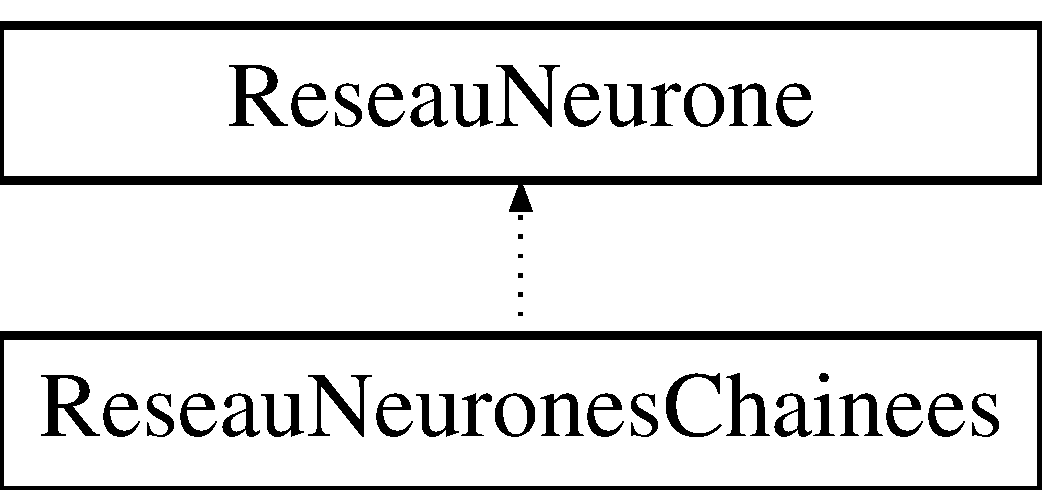
\includegraphics[height=2.000000cm]{classReseauNeuronesChainees}
\end{center}
\end{figure}


La documentation de cette classe a été générée à partir du fichier suivant :\begin{DoxyCompactItemize}
\item 
/home/cocouf/Documents/gm4/gm11-\/neurones/src/ReseauNeuronesChainees.h\end{DoxyCompactItemize}

\hypertarget{classReseauNeuronesCouches}{
\section{Référence de la classe ReseauNeuronesCouches}
\label{classReseauNeuronesCouches}\index{ReseauNeuronesCouches@{ReseauNeuronesCouches}}
}
Graphe d'héritage de ReseauNeuronesCouches:\begin{figure}[H]
\begin{center}
\leavevmode
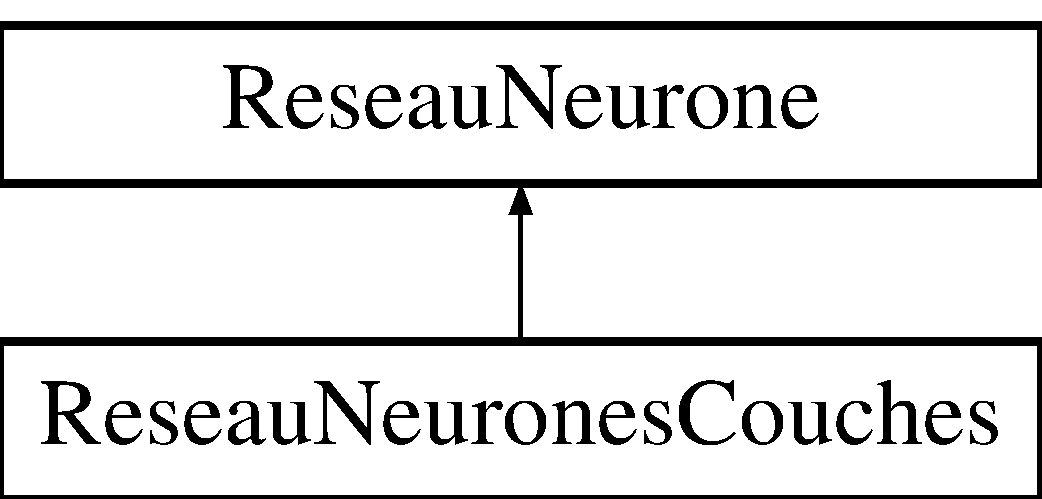
\includegraphics[height=2.000000cm]{classReseauNeuronesCouches}
\end{center}
\end{figure}
\subsection*{Fonctions membres publiques}
\begin{DoxyCompactItemize}
\item 
\hyperlink{classReseauNeuronesCouches_aed302a8c6aacaa7930bfd82096b4f963}{ReseauNeuronesCouches} (int nbNeuronesParCouche, int nbCouches)
\item 
\hyperlink{classReseauNeuronesCouches_a5647e91acb7d767a6ef3adc5a47b2f1e}{ReseauNeuronesCouches} (vector$<$ int $>$ nbNeuronesParCouche)
\item 
\hyperlink{classReseauNeuronesCouches_a7fe22661aa7ecb0cd959968a6521efba}{ReseauNeuronesCouches} (const \hyperlink{classReseauNeuronesCouches}{ReseauNeuronesCouches} \&u)
\item 
bool \hyperlink{classReseauNeuronesCouches_a22f5c01ae1f95cba98cc78f08729ea52}{chargerReseau} (string path)
\begin{DoxyCompactList}\small\item\em Cette méthode permet de charger un réseau lu dans un fichier. \end{DoxyCompactList}\item 
bool \hyperlink{classReseauNeuronesCouches_af2506fed92099704b3da33dcdbb534a7}{sauvegarderReseau} (string path)
\begin{DoxyCompactList}\small\item\em Cette méthode permet de sauvegarder un réseau dans un fichier. \end{DoxyCompactList}\item 
vector$<$ double $>$ \hyperlink{classReseauNeuronesCouches_ad2cb2070ae32e8772bf82e6d06221bdd}{calculerResultat} (vector$<$ double $>$ valeurEntree)
\begin{DoxyCompactList}\small\item\em Cette méthode permet de calculer le résultat sur la couche de sortie. \end{DoxyCompactList}\item 
void \hyperlink{classReseauNeuronesCouches_ad368a99d25583fd49d384516dacb3062}{apprendre} (vector$<$ double $>$ $\ast$entrees, vector$<$ double $>$ $\ast$valeursAttendues, int n)
\begin{DoxyCompactList}\small\item\em Cette méthode permet de réaliser l'apprentissage complet à partir d'un jeu de données. \end{DoxyCompactList}\end{DoxyCompactItemize}
\subsection*{Amis}
\begin{DoxyCompactItemize}
\item 
\hypertarget{classReseauNeuronesCouches_a755d7d72d9539f75e09ce6a61ce5e702}{
class {\bfseries Test\_\-ReseauNeuronesCouche}}
\label{classReseauNeuronesCouches_a755d7d72d9539f75e09ce6a61ce5e702}

\end{DoxyCompactItemize}


\subsection{Documentation des constructeurs et destructeur}
\hypertarget{classReseauNeuronesCouches_aed302a8c6aacaa7930bfd82096b4f963}{
\index{ReseauNeuronesCouches@{ReseauNeuronesCouches}!ReseauNeuronesCouches@{ReseauNeuronesCouches}}
\index{ReseauNeuronesCouches@{ReseauNeuronesCouches}!ReseauNeuronesCouches@{ReseauNeuronesCouches}}
\subsubsection[{ReseauNeuronesCouches}]{\setlength{\rightskip}{0pt plus 5cm}ReseauNeuronesCouches::ReseauNeuronesCouches (
\begin{DoxyParamCaption}
\item[{int}]{nbNeuronesParCouche, }
\item[{int}]{nbCouches}
\end{DoxyParamCaption}
)}}
\label{classReseauNeuronesCouches_aed302a8c6aacaa7930bfd82096b4f963}
Ceci est le constructeur de la classe reseau neurone par couche. 
\begin{DoxyParams}{Paramètres}
{\em nbNeuronesParCouche} & le nombre de neurones par couche (dans ce cas le nombre de neurones par couche est fixé) \\
\hline
{\em nbCouches} & le nombre de couches \\
\hline
\end{DoxyParams}
\hypertarget{classReseauNeuronesCouches_a5647e91acb7d767a6ef3adc5a47b2f1e}{
\index{ReseauNeuronesCouches@{ReseauNeuronesCouches}!ReseauNeuronesCouches@{ReseauNeuronesCouches}}
\index{ReseauNeuronesCouches@{ReseauNeuronesCouches}!ReseauNeuronesCouches@{ReseauNeuronesCouches}}
\subsubsection[{ReseauNeuronesCouches}]{\setlength{\rightskip}{0pt plus 5cm}ReseauNeuronesCouches::ReseauNeuronesCouches (
\begin{DoxyParamCaption}
\item[{vector$<$ int $>$}]{nbNeuronesParCouche}
\end{DoxyParamCaption}
)}}
\label{classReseauNeuronesCouches_a5647e91acb7d767a6ef3adc5a47b2f1e}
Ceci est le constructeur de la classe reseau neurone par couche. 
\begin{DoxyParams}{Paramètres}
{\em nbNeuronesParCouche} & un tableau qui contient le nombre de neurone de chaque couche (ce nombre peut varier d'une couche à l'autre). Le nombre de couches retenues est la taille du tableau. \\
\hline
\end{DoxyParams}
\hypertarget{classReseauNeuronesCouches_a7fe22661aa7ecb0cd959968a6521efba}{
\index{ReseauNeuronesCouches@{ReseauNeuronesCouches}!ReseauNeuronesCouches@{ReseauNeuronesCouches}}
\index{ReseauNeuronesCouches@{ReseauNeuronesCouches}!ReseauNeuronesCouches@{ReseauNeuronesCouches}}
\subsubsection[{ReseauNeuronesCouches}]{\setlength{\rightskip}{0pt plus 5cm}ReseauNeuronesCouches::ReseauNeuronesCouches (
\begin{DoxyParamCaption}
\item[{const {\bf ReseauNeuronesCouches} \&}]{u}
\end{DoxyParamCaption}
)}}
\label{classReseauNeuronesCouches_a7fe22661aa7ecb0cd959968a6521efba}
Ceci est le constructeur par recopie de la classe reseau neurone par couche. 

\subsection{Documentation des fonctions membres}
\hypertarget{classReseauNeuronesCouches_ad368a99d25583fd49d384516dacb3062}{
\index{ReseauNeuronesCouches@{ReseauNeuronesCouches}!apprendre@{apprendre}}
\index{apprendre@{apprendre}!ReseauNeuronesCouches@{ReseauNeuronesCouches}}
\subsubsection[{apprendre}]{\setlength{\rightskip}{0pt plus 5cm}void ReseauNeuronesCouches::apprendre (
\begin{DoxyParamCaption}
\item[{vector$<$ double $>$ $\ast$}]{entrees, }
\item[{vector$<$ double $>$ $\ast$}]{valeursAttendues, }
\item[{int}]{n}
\end{DoxyParamCaption}
)}}
\label{classReseauNeuronesCouches_ad368a99d25583fd49d384516dacb3062}


Cette méthode permet de réaliser l'apprentissage complet à partir d'un jeu de données. 


\begin{DoxyParams}{Paramètres}
{\em entrees} & liste des entrées pour le jeu d'apprentissage. \\
\hline
{\em valeursAttendues} & les valeurs attendues en sortie pour chacunes de ses entrées. \\
\hline
{\em n} & la taille de l'échantillon d'apprentissage. \\
\hline
\end{DoxyParams}


Réimplémentée à partir de \hyperlink{classReseauNeurone_ad29ad61f93877aaf2ee930106d46e48b}{ReseauNeurone}.

\hypertarget{classReseauNeuronesCouches_ad2cb2070ae32e8772bf82e6d06221bdd}{
\index{ReseauNeuronesCouches@{ReseauNeuronesCouches}!calculerResultat@{calculerResultat}}
\index{calculerResultat@{calculerResultat}!ReseauNeuronesCouches@{ReseauNeuronesCouches}}
\subsubsection[{calculerResultat}]{\setlength{\rightskip}{0pt plus 5cm}vector$<$ double $>$ ReseauNeuronesCouches::calculerResultat (
\begin{DoxyParamCaption}
\item[{vector$<$ double $>$}]{valeurEntree}
\end{DoxyParamCaption}
)}}
\label{classReseauNeuronesCouches_ad2cb2070ae32e8772bf82e6d06221bdd}


Cette méthode permet de calculer le résultat sur la couche de sortie. 

\begin{DoxyReturn}{Renvoie}
la valeur des résultats. 
\end{DoxyReturn}


Réimplémentée à partir de \hyperlink{classReseauNeurone_add3e1d607bc614ca36b0375daf546106}{ReseauNeurone}.

\hypertarget{classReseauNeuronesCouches_a22f5c01ae1f95cba98cc78f08729ea52}{
\index{ReseauNeuronesCouches@{ReseauNeuronesCouches}!chargerReseau@{chargerReseau}}
\index{chargerReseau@{chargerReseau}!ReseauNeuronesCouches@{ReseauNeuronesCouches}}
\subsubsection[{chargerReseau}]{\setlength{\rightskip}{0pt plus 5cm}bool ReseauNeuronesCouches::chargerReseau (
\begin{DoxyParamCaption}
\item[{string}]{path}
\end{DoxyParamCaption}
)\hspace{0.3cm}{\ttfamily  \mbox{[}virtual\mbox{]}}}}
\label{classReseauNeuronesCouches_a22f5c01ae1f95cba98cc78f08729ea52}


Cette méthode permet de charger un réseau lu dans un fichier. 


\begin{DoxyParams}{Paramètres}
{\em path} & une chaine de caractère décrivant le nom du fichier dans lequel est stocké le réseau. \\
\hline
\end{DoxyParams}
\begin{DoxyReturn}{Renvoie}
Si oui ou non le chargement s'est bien déroulé. 
\end{DoxyReturn}


Implémente \hyperlink{classReseauNeurone_ac2bccb9c9106a989960246e8f173d93a}{ReseauNeurone}.

\hypertarget{classReseauNeuronesCouches_af2506fed92099704b3da33dcdbb534a7}{
\index{ReseauNeuronesCouches@{ReseauNeuronesCouches}!sauvegarderReseau@{sauvegarderReseau}}
\index{sauvegarderReseau@{sauvegarderReseau}!ReseauNeuronesCouches@{ReseauNeuronesCouches}}
\subsubsection[{sauvegarderReseau}]{\setlength{\rightskip}{0pt plus 5cm}bool ReseauNeuronesCouches::sauvegarderReseau (
\begin{DoxyParamCaption}
\item[{string}]{path}
\end{DoxyParamCaption}
)\hspace{0.3cm}{\ttfamily  \mbox{[}virtual\mbox{]}}}}
\label{classReseauNeuronesCouches_af2506fed92099704b3da33dcdbb534a7}


Cette méthode permet de sauvegarder un réseau dans un fichier. 


\begin{DoxyParams}{Paramètres}
{\em path} & une chaine de caractère décrivant le nom du fichier dans lequel on stocke le réseau. \\
\hline
\end{DoxyParams}
\begin{DoxyReturn}{Renvoie}
Si oui ou non la sauvegarde s'est bien déroulée. 
\end{DoxyReturn}


Implémente \hyperlink{classReseauNeurone_a33c828f2e2b7a190eff04c613707a9d4}{ReseauNeurone}.



La documentation de cette classe a été générée à partir des fichiers suivants :\begin{DoxyCompactItemize}
\item 
/home/cocouf/Documents/gm4/gm11-\/neurones/src/ReseauNeuronesCouches.h\item 
/home/cocouf/Documents/gm4/gm11-\/neurones/src/ReseauNeuronesCouches.cpp\end{DoxyCompactItemize}

\hypertarget{classSigmoide}{
\section{Référence de la classe Sigmoide}
\label{classSigmoide}\index{Sigmoide@{Sigmoide}}
}


class Sigmoïde -\/  




{\ttfamily \#include $<$Sigmoide.h$>$}

Graphe d'héritage de Sigmoide:\begin{figure}[H]
\begin{center}
\leavevmode
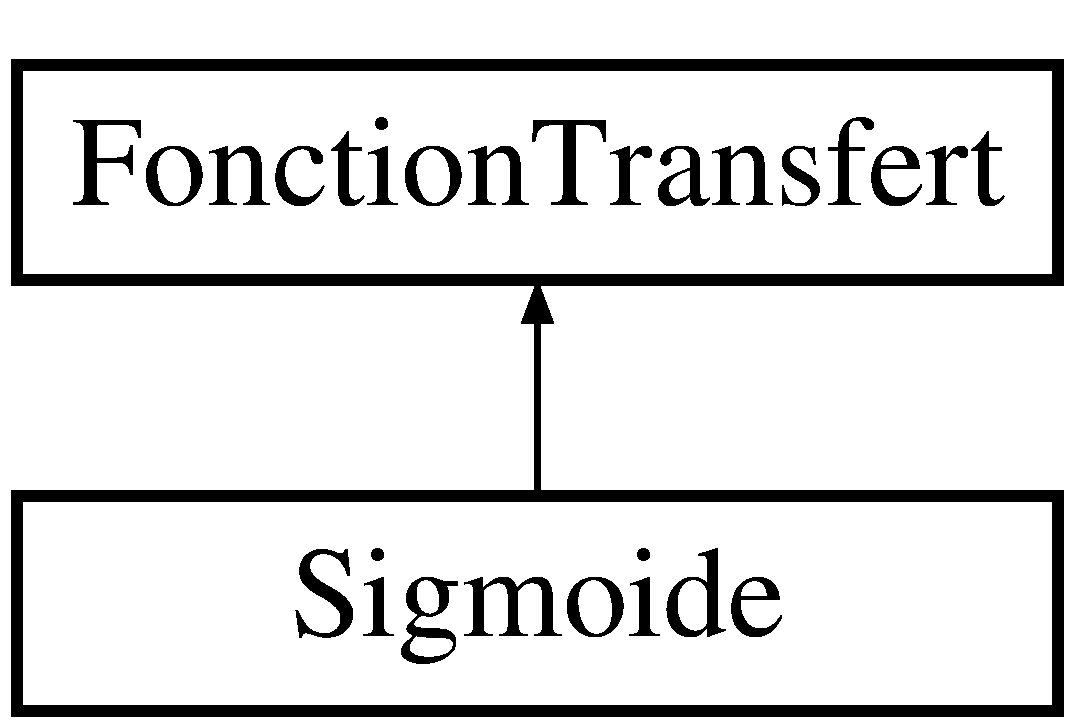
\includegraphics[height=2.000000cm]{classSigmoide}
\end{center}
\end{figure}
\subsection*{Fonctions membres publiques statiques}
\begin{DoxyCompactItemize}
\item 
\hypertarget{classSigmoide_a3bf746fe163bdd5180fb2f3cbe95ecc3}{
static double {\bfseries f} (double x)}
\label{classSigmoide_a3bf746fe163bdd5180fb2f3cbe95ecc3}

\item 
\hypertarget{classSigmoide_accaa035158e86d4f22cdc5b5db3ae3b3}{
static double {\bfseries f\_\-inverse} (double x)}
\label{classSigmoide_accaa035158e86d4f22cdc5b5db3ae3b3}

\item 
\hypertarget{classSigmoide_ae3d4858677b26fabebade43d37874a82}{
static double {\bfseries f\_\-derive} (double x)}
\label{classSigmoide_ae3d4858677b26fabebade43d37874a82}

\end{DoxyCompactItemize}


\subsection{Description détaillée}
class Sigmoïde -\/ 

La documentation de cette classe a été générée à partir des fichiers suivants :\begin{DoxyCompactItemize}
\item 
/home/cocouf/Documents/gm4/gm11-\/neurones/src/Sigmoide.h\item 
/home/cocouf/Documents/gm4/gm11-\/neurones/src/Sigmoide.cpp\end{DoxyCompactItemize}

\printindex
\end{document}
